\section{Obranné mechanismy proti analýze softwaru}

Postupy obrany proti analýze využívá jak běžně užívaný software pro účel ochrany duševního vlastnictví, tak i škodlivý kód k znesnadnění odhalení. Tato ochrana počítačových programů může být provedena více způsoby. Těmito způsoby se dále zabývá tato kapitola.

%%% MALWARE
%%% Ochrana programu proti crackování atd
%%% DRM

\paragraph*{Ochrana duševního vlastnictví}
Vlastníci práv a autoři softwaru využívají různé techniky, kterými se snaží ochránit své duševní vlastnictví například algoritmy (komunikační protokol programu Skype). Často se však také jedná o multimediální obsah, který obsahuje nějakou ochranu. Příkladem mohou být počítačové hry, u kterých se vydavatelé snaží ochránit hru před tzv. crackingem, kdy se nejrůznější organizace snaží prolomit a odstranit ochranu hry. 

%% Multimediální obsah, snaží se ochranit software, filmy, hudbu aby nebylo možné jednoduše prolomit ochranu k sw
%% Skrytí myšlenek před konkurencí - Skype
%% DRM ochrana médií
%% https://en.wikipedia.org/wiki/Denuvo - odolavalo fest dlouho

\paragraph*{Malware}

Autoři malwaru se stále snaží vymýšlet nové techniky ukrytí malwaru a znemožnění nebo alespoň ztížení jeho analýzy. 
%% chcou být o krok napřed
%% neodhalitelní

\subsection{Anti-debug}
\label{anti_debug}

Tento způsob ochrany brání ladění neboli debugovaní programu. Implementují ho často jak~legitimní aplikace, které potřebuji utajit své know-how, tak i tvůrci malwaru. Existuje mnoho způsobů jak přítomnost debuggeru detekovat a případně ho blokovat. Mezi ty nejpopulárnější patří následující \cite{sikorski2012practical}.

\paragraph*{Windows API}

Microsoft Windows obsahuje ve svém API několik zpusobů jak debugger detekovat. Některé funkce byly navrženy přímo pro detekci debuggeru, některé zase pro jiné účely, ale lze je pro detekci použít.

Nejjednodušším způsobem je použít metodu \emph{IsDebuggerPresent}. Tato metoda sleduje strukturu PEB, která obsahuje informace o aktuálním procesu, včetně pole \emph{IsDebugged}. Pokud je~toto pole nastaveno na nulu, debugger není přítomen. V opačném případě je program spuštěn v~debug režimu.

Obdobným způsobem můžeme použít metodu \emph{CheckRemoteDebuggerPresent}, která funguje na podobném principu. Rozdíl spočívá v tom, že tato funkce byla navržena ke sledování debuggu cizího (vzdáleného) procesu. Lze ji však nastavit tak, aby plnila i tento úkol.

Další možností je funkce \emph{NtQueryInformationProcess}. Metoda opět slouží k získání informací o požadovaném procesu. Prvním parametrem funkce je ukazatel na proces. Dalším parametrem je pak možné nastavit typ získané informace. 

Alternativním řešením bez sledování struktury PEB může být \emph{OutputDebugString}. Funkce slouží k odeslání řetězce na výstup debuggeru. Pokud však debugger nebude přítomen a chybový kód bude nastaven pomocí funkce \emph{SetLastError} bude po zavolání \emph{OutputDebugString} na výstupu chybový kód funkce \emph{OutputDebugString}. V případě, že by debugger přítomen byl, na výstupu bude chybový kód, který byl nastaven přes funkci \emph{SetLastError}.

\paragraph*{Detekce chování debuggeru}

Další variantou této ochrany je detekce základní funkce debuggeru a to breakpointu \cite{deepinstrinct_antidebug}. Breakpoint slouží analytikovi k zastavení kódu a funguje na principu vložení instrukce \emph{INT 3} do kódu. Instrukce \emph{INT 3} slouží k vyvolání breakpointu neboli přerušení. Malware však může skenovat sám sebe a hledat tuto instrukci v kódu. Případně vytvářet za~běhu kontrolní součet nebo hash aby zjistil, zda nebylo zasaženo do kódu.


\paragraph*{TLS callback}
%https://www.deepinstinct.com/2017/12/27/common-anti-debugging-techniques-in-the-malware-landscape/
%https://docs.microsoft.com/cs-cz/cpp/parallel/thread-local-storage-tls?view=vs-2019
TLS je místní paměťový prostor v rámci jednoho vlákna, kde může dané vlákno ukládat svá data \cite{msdocs_tls}. Tato vlastnost může být zneužita tak, že ještě před vstupním bodem programu, kdy je inicializováno vlákno aplikace, se zavolá potřebná funkce \cite{deepinstrinct_antidebug}.


\paragraph*{Zneužití zranitelnosti debuggeru}
%https://exchange.xforce.ibmcloud.com/vulnerabilities/16711
Stejně jako každý software i debuggery mohou obsahovat zranitelnosti. Autoři malwaru si to samozřejmě uvědomují a této skutečnosti zneužívají. Příkladem může být chyba známého a používaného debuggeru OllyDbg ve verzi 1.1 \cite{CVE-2004-0733}, která umožňovala aplikaci shodit pomocí formátovacího řetězce, zaslaného přes Windows API metodou \emph{OutputDebugString}.
\subsection{Obfuskace}
%https://researchspace.auckland.ac.nz/bitstream/handle/2292/3491/TR148.pdf
%https://searchsoftwarequality.techtarget.com/definition/obfuscation
%https://securityintelligence.com/an-example-of-common-string-and-payload-obfuscation-techniques-in-malware/
\label{obfuskacni_metody}

Obfuskace je transformace kódu takovým způsobem, aby bylo zamezeno či alespoň znesnadněno analyzování daného kódu člověkem, přičemž funkčnost kódu setrvává \cite{13355040520180901} \cite{Obfuscation}. Je možno využít různé techniky. Tyto techniky mohou být například: 

\paragraph*{Obfuskace struktury}
Tato transformace se řadí mezi ty nejjednoduší. Mění strukturu zdrojového kódu programu. Přeměna je jednosměrná a již nelze získat původní zdrojový kód. Při~této obfuskaci jsou odstraněny komentáře, mění se formátování (např. minifikací - odstranění nepotřebných znaků ze zdrojového kódu), je provedena změna názvů metod ( metoda() = \_a()) a proměnných ( string heslo = string a ).

%% transformace mění strukturu programu
%% jsou odstraněny komentáře v kódu
%% mění se formátování, název metod/funkcí ( funkce() = _a() ) / proměnných ( heslo = a )
%% jednosměrné , nelze získat původní kód
\paragraph*{Datová obfuskace}
%https://researchspace.auckland.ac.nz/bitstream/handle/2292/3491/TR148.pdf¨
%https://www.paladion.net/blogs/code-obfuscation-part-2-obfuscating-data-structures
%https://medium.com/better-programming/code-obfuscation-introduction-to-code-obfuscation-part-1-93a6797349b0
%https://selab.fbk.eu/ceccato/papers/2015/spro2015.pdf

Metoda datové obfuskace pracuje s maskováním datových struktur pomocí jejich přeměny na jiné sémanticky však stejné. Tento druh obfuskace se často používá pro skrytí citlivých informací. V případě malwaru se může jednat o důležité informace jako například doménové jméno či IP adresy CnC serveru, šifrovací klíče apod. Tyto transformace mohou být provedeny několika způsoby a jsou popsány níže \cite{DataObfuscation}.

\subparagraph*{Nahrazení statických dat}
%% Změna datových struktur
%% převod proměnných na metody
%% globalizace

Nejjednodušší způsob obfuskace statických dat je nahrazení metodou. Data jsou nahrazena kódem, který je bude dynamicky generovat. Účinnost tohoto řešení se zvyšuje s počtem volaných funkcí, jejichž volání je náhodně rozloženo do toku programu \cite{DataObfuscation}. Pro zmatení reverzního inženýra je možné přidat také několik výstupů, ke kterým při~normálním běhu programu nedojde.

Tuto metodu lze vidět na následující ukázce č. \ref{src:StaticData}. Statická data byla nahrazena jednoduchým \emph{switchem}, který podle čísla vstupu vrátí požadovanou hodnotu.

\noindent
\begin{minipage}[t]{1\textwidth}
    \lstinputlisting[basicstyle=\footnotesize,caption={Generování statických dat},label=src:StaticData]{zdrojaky/obfuskace/staticka-data.cs}
\end{minipage}

\subparagraph*{Rozdělení proměnných}
%% Změna z a=123 na a = 100 ; b = 20; c = 3 ; a + b + c 

Velmi účinnou technikou obfuskace proměnných je jejich rozdělení a to nejlépe za použití různých datových typů \cite{DataObfuscation2}. Cílem je zmást reverzního inženýra velkým množstvím použitých proměnných. \par Síla a odolnost této transformace roste s počtem použitých proměnných a různorodosti jejich typů.

Následující ukázka kódu č. \ref{src:VariableJoining1} a \ref{src:VariableJoining2} prezentuje tuto metodu. Původní proměnnou je možné vidět v prvním výpisu č. \ref{src:VariableJoining1} obfuskvanou proměnnou pak v ukázce č. \ref{src:VariableJoining2}. Pokud bychom definice proměnných proložili sekvencemi vykonávaného kódu docílili bychom ještě lepšího výsledku.

%\ref{ref:SkladaniPromenne}

%%%%%%%%%%%%%%% Výstup %%%%%%%%%%%%%
%\begin{center}	
    %\label{src:SkladaniPromenne}
    \noindent
    \begin{minipage}[t]{1\textwidth}
        \noindent
        \centering
        \lstinputlisting[basicstyle=\footnotesize,caption={Proměnná bez obfuskace},label=src:VariableJoining1]{zdrojaky/obfuskace/skladani-promenne1.cs}
    \end{minipage}
    \newline
    %\hfill
    \begin{minipage}[t]{1\textwidth}
        \lstinputlisting[basicstyle=\footnotesize,caption={Obfuskovaná proměnná},label=src:VariableJoining2]{zdrojaky/obfuskace/skladani-promenne2.cs}
    \end{minipage}
%\end{center}
%%%%%%%%%%%%%%%%%%%%%%%%%%%%%%%%%%%%%%


\subparagraph*{Globalizace proměnné}
%%% TODO
Máme-li funkce, například FA() a FB(), jež používají stejnou lokální proměnnou, definovanou ve svém těle a nevykonávají-li se souběžně, můžeme takovouto proměnnou deklarovat globálně a bude tak sdílena mezi oběma funkcemi \cite{DataObfuscation}. 

\subparagraph*{Sloučení proměnných}
%% sloučení více proměnných do jedné třeba 2 32b čísla mohou být jako 64b

Další metodou obfuskace proměnných je jejich sloučení do jedné. Příkladem mohou být dvě 32-bitová čísla X a Y. Tato čísla mohou být sloučena do jednoho 64-bitového dle následujícího vzorce \ref{src:SlouceniPromennychDo64b} \cite{DataObfuscation}.

\begin{equation}
    \label{src:SlouceniPromennychDo64b}
    V = 2^{32} * Y + X
\end{equation}

Odolnost této přeměny je malá, protože deobfuskátor může odhadnout, že proměnná~V se skládá ze dvou proměnných a to zkoumáním aritmetických operací.


\subparagraph*{Šifrování a kódování}
%% TODO
%% Zašifruji data
%%https://medium.com/@bromiley/malware-monday-obfuscation-f65239146db0

Další možností obfuskace dat je jejich šifrování popřípadě jejich kódování. Šifrovány mohou být buď jednotlivé části kódu nebo celé sekce spustitelného souboru \cite{sevagas_2014}. Zašifrovaná data jsou následně při spuštění dešifrována \cite{guardsquare_2019}. Tím je zaručeno, že program funguje tak jak byl vytvořen.

Často je možné se setkat s šifrováním pomocí bitové funkce \emph{XOR} nebo kódováním do \emph{Base64}. Takovéto zakrytí dat může oddálit odhalení skutečného obsahu, protože nemusí být na první pohled patrné, že jsou data šifrována nebo kódována.


%Oproti šifrování, užívaném například v síťové komunikaci, se používají také často již prolomené šifry. 
%Můžeme se setkat s šifrováním pomocí bitové funkce XOR nebo kódovaní do Base64. Takovéto zakrytí dat může prodloužit odhalení skutečného obsahu, protože při spuštění se kód prvně dešifruje a 

        %http://www.hjp.at/doc/rfc/rfc4648.html#sec_4
        %https://iopscience.iop.org/article/10.1088/1742-6596/1007/1/012003/pdf
        
        
Kódování \emph{Base64} bylo původně navrženo pro přenos příloh v emailové komunikaci a je~součásti standardu MIME \cite{sikorski2012practical}. Kódování \emph{Base64} umožňuje převést binární data na ASCII řetězec~a, jak~značí číslo 64 v názvu kódování, používá se právě 64 (resp. 65) znaků US-ASCII. Znaky užívané kódováním jsou a-z, A-Z, 0-9, +, / a = pro zarovnání délky \cite{RFC4648}.

Implementace do vlastního programu je velmi jednoduchá a většina moderních programovacích jazyků už toto kódování umožňuje. Útočnici (autoři malwaru) tak často využívají toto kódování ke skrytí závadného kódu nebo dat. 

%check this:
%Kódování pomocí Base64 umožňuje převést binární data na ASCII řetězec. Tím pádem lze přenést binární data jakoukoliv cestou. Původně bylo navrženo pro přenos příloh v emailové komunikaci. 

% komplikuje to zjištění co je obsahem
% umožňuje použít vlastní abecedu
% má popsaný algoritmus přesně (RFC)
% 

Šifrování pomocí exkluzivní disjunkce (\emph{XOR}) je velmi oblíbeným způsobem šifrováním mezi tvůrci malwaru \cite{sikorski2012practical}, protože se jedná o oboustrannou funkci, není potřeba implementovat různé algoritmy pro šifrování a dešifrování \ref{fig:XorSifrovani}. Klíčem je vždy proud bitů \cite{kpb_ochodkova2019}.

\begin{figure}[!ht]
    \caption{De/šifrování pomocí XOR}
    \centering
    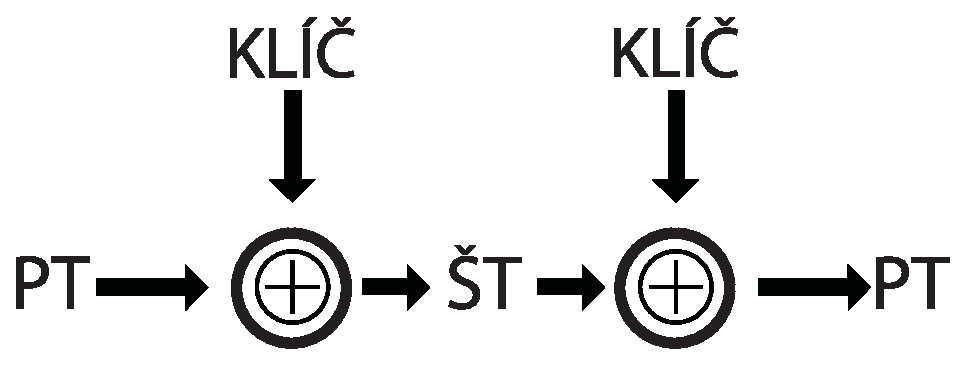
\includegraphics[width=75mm,scale=0.5]{Figures/obrazky/pt-st-pt-xorsifra.eps}
    \label{fig:XorSifrovani}
\end{figure}
    
%Šifrování pomocí exkluzivní disjunkce je velmi jednoduché na implementaci a protože se jedná o oboustrannou funkci, odpadá nutnost impl. Klíčem je vždy proud bitů. 
 
 
 
 % oboustranná funkce P -> C -> P
\paragraph*{Obfuskace běhu programu}
Tato transformace je využívána za účelem maskování posloupnosti kódu. Provádí se například záměnou pořadí prováděných instrukcí pomocí podmíněných skoků, vloženým nahodilým mrtvým kódem atd. \cite{13355040520180901}.
%https://www.paladion.net/blogs/code-obfuscation-part-3-hiding-control-flows

%%%%%%%%%%%%%%%%%%%%%%%%%%%%%%%%%%%%%%

\subparagraph*{Změna pořadí prováděného kódu}
Tento typ obfuskace spočívá v tom, že jsou provedeny skoky mezi jednotlivými částmi programu, které jsou náhodně rozmístěny. Přestože probíhají skoky, chování počítačového programu se nezmění. Tato metoda je v podstatě jednoduchá nicméně v delším kódu komplikuje analýzu pořadí prováděných operací \cite{13355040520180901}. 

Princip prezentuje následující výstup kódu č. \ref{src:ChangedOrder1} a \ref{src:ChangedOrder2}. Kód byl rozdělen do několika části (\emph{.start, .end a .continue}) následně byl náhodně rozmísten. Podmíněné skoky (\emph{JMP}) pak zajistí aby došlo k vykonání kódu ve správném pořadí.

%%%%%%%%%%%%%%% Výstup %%%%%%%%%%%%%
\noindent
\begin{minipage}[t]{.475\textwidth}
    \lstinputlisting[basicstyle=\footnotesize,label=src:ChangedOrder1,caption={Původní kód funkce bez obfuskace}]{zdrojaky/obfuskace/zmena-poradi-kodu1.asm}
\end{minipage}
\hfill
\begin{minipage}[t]{.475\textwidth}
    \lstinputlisting[basicstyle=\footnotesize,label=src:ChangedOrder2,caption={Obfuskovaný kód funkce}]{zdrojaky/obfuskace/zmena-poradi-kodu2.asm}
\end{minipage}
%%%%%%%%%%%%%%%%%%%%%%%%%%%%%%%%%%%%%%

\subparagraph*{Vložení nahodilého kódu}
Tato technika obfuskace je založena na vložení mrtvého nebo nepodstatného kódu do programu. Využívají ji především útočnici, protože pomocí této metody lze vytvořit novou verzi programu, která se chová stejně. Účel spočívá především ve zmatení detekce antiviry, protože vložený kód změní signaturu programu (známé signatury jsou využívány pro rychlou detekci malwaru) \cite{13355040520180901}. 

Ukázka následujících výpisu č. \ref{src:RandomCodeInserted1} a \ref{src:RandomCodeInserted2} prezentuje rozdíl hlavně v délce kódu. Do kódu bylo vloženo několik skoků pomocí \emph{JMP} a instrukcí \emph{NOP}, která nevykonává žádnou operaci.

%%%%%%%%%%%%%%% Výstup %%%%%%%%%%%%%
\noindent
\begin{minipage}[t]{.475\textwidth}
    \lstinputlisting[basicstyle=\footnotesize,label=src:RandomCodeInserted1,caption={Původní kód bez obfuskace vloženého kódu}]{zdrojaky/obfuskace/vlozeni-nahodileho-kodu1.asm}
\end{minipage}
\hfill
\begin{minipage}[t]{.475\textwidth}
    \lstinputlisting[basicstyle=\footnotesize,label=src:RandomCodeInserted2,caption={Kód funkce po obfuskaci}]{zdrojaky/obfuskace/vlozeni-nahodileho-kodu2.asm}
\end{minipage}
%%%%%%%%%%%%%%%%%%%%%%%%%%%%%%%%%%%%%%

\subparagraph*{Nahrazení ekvivalentem}
Díky nahrazení části kódu ekvivalentem lze provádět stejnou funkcionalitu programu různými způsoby. Tím je možné dosáhnout změny signatury, což způsobí vyšší náročnost detekce malwaru, takto vznikají nové verze u nichž je potřeba uchovat signaturu každé nové jedinečné verze \cite{13355040520180901}. 

Následující výpisy kódu č. \ref{src:ReplacedByEkvivalent1} a \ref{src:ReplacedByEkvivalent2} prezentují tuto metodu. Kód se liší ve dvou podstatných instrukcích, jež vykonávají ekvivalentní funkci a to instrukce \emph{test} nahrazena ekvivalentem \emph{cmp} a instrukce \emph{inc} nahrazena \emph{add}.

%%%%%%%%%%%%%%% Výstup %%%%%%%%%%%%%
\noindent
\begin{minipage}[t]{.475\textwidth}
    \lstinputlisting[basicstyle=\footnotesize,label=src:ReplacedByEkvivalent1,caption={Kód před nahrazením}]{zdrojaky/obfuskace/nahrazeni-ekvivalentem1.asm}
\end{minipage}
\hfill
\begin{minipage}[t]{.475\textwidth}
    \lstinputlisting[basicstyle=\footnotesize,label=src:ReplacedByEkvivalent2,caption={Kód po nahrazení}]{zdrojaky/obfuskace/nahrazeni-ekvivalentem2.asm}
\end{minipage}
%%%%%%%%%%%%%%%%%%%%%%%%%%%%%%%%%%%%%%

%\subparagraph*{Packing kódu}

\subsection{Komprese}

Cílem komprese spustitelných souborů je zmenšit celkovou velikost kódu a sekcí s daty. Původní spustitelný soubor se nahradí souborem novým. Tento nový soubor obsahuje program pro dekompresi a původní spustitelný soubor jež je komprimovaný.  Pří spuštění se původní soubor nejdřív dekomprimuje do paměti a následně se spustí \cite{golchikov_2002}.

Běžné formáty spustitelných souborů, jako PE, ELF atp. v základu kompresi nepodporují. Proto v době, kdy byl nedostatek paměti a malá velikost spustitelných souborů byla tedy nutností, začala tak vznikat různá řešení pro kompresi spustitelných souborů.

V současnosti se však komprese využívá spíše z důvodu možnosti skrýt obsah spustitelného souboru bez jeho dekomprese.

%https://reverseengineering.stackexchange.com/questions/14288/what-is-executable-compression
%https://patentimages.storage.googleapis.com/90/80/a7/7bd0343cf32f90/US20020112158A1.pdf


% DEKOMPRESE? %TODO DEKOMPRESE?
\subsection{Packery}
\label{packers}

Při použití packingu dochází k zabalení původního programu nebo jeho části a to pomocí packeru nad binárními daty. Může docházet k zašifrování nebo kompresi. Packer nahradí původní program nebo jeho část tzv. unpackerem. Při spuštění kódu se nejprve provede tzv. unpacking do paměti a následně se kód spustí \cite{diff_packers}. Tvůrci malwaru využívají tuto techniku packování velmi často, za~účelem ztížení a časové prodloužení analýzy kódu reverzním inženýrem \cite{HoonKang2011}.

% Kompresory, bundlery, kodéry, protektory

%% EXAMPLE IMAGE

Při svém procesu mohou zároveň provádět kompresi, obfuskaci, šifrování nebo přidat jinou funkcionalitu pro ztížení reverzní analýzy \cite{packers_2010}. Druhy packerů si popíšeme v následujícím textu, součástí bude porovnání několika packerů viz tabulka č. \ref{table:packeryTabulka}. Některé packery, jež jsou porovnávaný jsou veřejně dostupné a mají také otevřený zdrojový kód (UPX, Obfuscator, ConfuserEX). Otevřený kód může nahrávat reverzním analytikům, protože snáze zjistí jak packer funguje a mohou tak tedy kód případně snáze unpackovat. Existují však také komerční packery, které otevřeným kódem nedisponují a je těžší je analyzovat.

%https://gironsec.com/code/packers.pdf
%https://www.boxedapp.com/exe_bundle.html
%https://www.security-portal.cz/clanky/seznamte-se-%E2%80%93-morfismy-oligomorfismus-polymorfismus-metamorfismus

%%
\paragraph*{Rozšiřující}

\subparagraph*{Kompresory} Tento druh packeru slouží primárně k snížení velikosti spustitelného souboru. Před spuštěním se provede dekomprese do paměti a soubor se spustí \cite{diff_packers}.

\subparagraph*{Protektor} Cílem protektoru je ztížit analýzu kódu různými metodami jako anti-debug, anti-vm apod. a ochránit tak kód vůči reverzní analýze \cite{packers-malwarbytes}.

\subparagraph*{Kryptor}  Dalším druhem packeru je kryptor, jež provádí šifrování originálního souboru. Před spuštěním je nejprve dešifrován a následně spuštěn \cite{packers-malwarbytes}.

\subparagraph*{Bundler} Tato metoda packování umožňuje zabalit do jednoho souboru všechny potřebné soubory. Program se tedy na první pohled tváří, že neobsahuje žádné externí knihovny apod. \cite{diff_packers}. 

%%
\paragraph*{Transformující} %https://www.security-portal.cz/clanky/seznamte-se-%E2%80%93-morfismy-oligomorfismus-polymorfismus-metamorfismus

\subparagraph*{Virtualizátor} Virtualizátory převádí původní spustitelný kód do jazyku virtuálního stroje, který následně provádí vestavěný virtuální stroj \cite{diff_packers}. 

\subparagraph*{Mutátor} Převádí instrukce na alternativní (v rámci stejné platformy). Využívá se oligomorfismu \cite{diff_packers}.


%https://blog.malwarebytes.com/cybercrime/malware/2017/03/explained-packer-crypter-and-protector/
%https://www.mcafee.com/blogs/enterprise/malware-packers-use-tricks-avoid-analysis-detection/
%https://reverseengineering.stackexchange.com/questions/1779/what-are-the-different-types-of-packers

%https://archive.codeplex.com/?p=netdeob0
%https://en.wikipedia.org/wiki/Executable_compression

\noindent
\begin{table}[!ht]
    \centering
    \caption{Výběr některých packerů}
    \label{table:packeryTabulka}
    
    \begin{tabular}{|l|l|c|c|c|c|c|}
    \hline
        Název & Licence & x86-64 & Komprese & Obfuskace & Šifrování & Jiná \\
		\hline
		\hline
        UPX & GPL & \checkmark & \checkmark &  & & \\  \hline
        
        ASPack & Proprietární & x86 & \checkmark &  & & \\  \hline
        ASProtect & Proprietární & \checkmark & \checkmark &  & \checkmark & \checkmark \\  \hline
        Enigma Virtual Box & Proprietární & \checkmark & \checkmark & \checkmark & & \checkmark \\  \hline
        
        \hline
        Obfuscar & MIT & .NET & \checkmark & \checkmark & & \\ \hline
        ConfuserEx & MIT & .NET & \checkmark & \checkmark & \checkmark & \checkmark \\ \hline
    \end{tabular}
\end{table}

\subsection{Unpacking}
\label{unpackers}

Unpacking je proces, při kterém dochází k obnově původních zdrojových dat (kódu) z programu, jež byl zabalen jedním nebo vícero packery \cite{HoonKang2011}. Existují tří různé způsoby jak získat původní kód \cite{4639028}. A to buď pomocí ručního, statického nebo dynamický unpacking \cite{generic_unpacker}.

\paragraph*{Ruční unpacking}

Při ručním unpackingu reverzní analytik zkoumá jednotlivé vrstvy algoritmu, jímž byl kód šifrován, komprimován apod. A ručně se snaží o obnovu původních dat. Tato~technika je však velmi časově náročná, vyžaduje hlubší znalosti nižších vrstev OS a také znalost assembleru \cite{4639028}. 

\paragraph*{Statický unpacking}

Metoda statického unpackingu je vlastně způsob jak zautomatizovat unpacking známých packerů jako například kompresor UPX. Jde o rutinní operace, které provádí dekompresi, dešifrování apod. A umožňují tak snadno získat původní kód. Autoři malwaru však mohou mírně upravit packer nebo použít svůj vlastní a původní unpacker již nebude funkční \cite{4639028}. 

Tuto metodu také používají antivirové společnosti ve svém softwaru, aby urychlili detekci nových neznámých vzorků malwaru \cite{4639028}.

\paragraph*{Dynamický unpacking}

Zatímco statický unpacking se snaží nahradit proces packeru, jež~se stará o rozbalení a spuštění původní aplikace. Dynamický unpacker nechá rozbalení na původním programu. Unpacker nejdříve spustí zabalený program, nechá jej až se rozbalí do~paměti. A pak se snaží získat rozbalený kód z paměti a uložit do souboru \cite{generic_unpacker}.
\subsection{Anti-VM}
%https://www.cyberbit.com/blog/endpoint-security/anti-vm-and-anti-sandbox-explained/
Autoři malwaru jsou si plně vědomi využití izolovaného virtuálního prostředí při dynamické analýze. Proto do svých programů implementují techniky, jež detekují takové virtuální prostředí. V případě, že malware toto prostředí detekuje, může například deaktivovat svou funkčnost. V~případě statické analýzy, lze některé z těchto postupů odhalit.

Tvůrci škodlivého kódu, jež takovouto obranu implementují do svého programu, využívají znalostí o izolovaném prostředí. Tyto postupy jsou popsány níže \cite{cyberbit_2016}. (Při testování těchto funkcionalit byl použit VMware verze 15.5.1 a VirtualBox ve verzi 6.0.10)

%%%%%%%%%%%%%%%%%%%%%%%%%%%%%%%%%%%%%%
\subparagraph*{Instrukce CPU} 
%https://c9x.me/x86/html/file_module_x86_id_45.html
%https://cs.wikipedia.org/wiki/CPUID

Prvním způsobem jak detekovat virtuální prostředí je použití instrukce CPUID, která slouží k zjištění informaci o daném procesoru. 


Následující ukázka č. \ref{src:InstructionVM1} prezentuje instrukci CPUID pro zjištění, zda se program nachází ve virtuálním prostředí. Nejprve je nastaven registr EAX = 1 a následně je vykonána instrukce CPUID. Ta při nastaveném EAX na 1 vrátí do několika registrů (EAX-EDX) informace o procesoru. \cite{instruction_set_x86_cpuid} V tomto případě bude je předmětem zájmu registr ECX, který na 31. bitu obsahuje informaci, zda se jedná o hostitele nebo prostředí VM. Pokud bude tento bit nastaven na 0 jedná se o fyzický stroj, v opačném případě půjde o hosta \cite{cyberbit_2016}.

\noindent
\begin{minipage}[t]{1\textwidth}
    \lstinputlisting[basicstyle=\footnotesize,label=src:InstructionVM1,caption={Instrukce CPUID - Převzato z \cite{cyberbit_2016}}]{zdrojaky/antivm/cpuid.asm}
\end{minipage}

Obdobně lze využít instrukci CPUID viz ukázka č. \ref{src:InstructionVM1} k získání názvu hypervizoru virtualizačního softwaru. Postup je obdobný je potřeba nastavit registr EAX na hodnotu 40000000 a následně provést instrukci CPUID. Po provedení instrukce s tímto parametrem je následně nastavena hodnota registrů EAX, ECX a EDX.
Získané názvy jsou uvedeny v tabulce č. \ref{table:hypervisor_cpuid}.

\begin{table}[!ht]
    \centering
    \caption{Názvy získaných hypervizorů pomocí funkce CPUID}
    \label{table:hypervisor_cpuid}
    
    \begin{tabular}{|l|l|}
    \hline
        Hypervizor & Obsah registrů \\
		\hline
		\hline
        VirtualBox & VBoxVbox \\ \hline
        VMware     & VMwareVMware \\ \hline
        Hyper-V & Microsoft HV \\ \hline
    \end{tabular}
\end{table}


V případě VMware, může být použita také detekce díky tzv. VMWare Magic Number \cite{sikorski2012practical} (viz~ukázka č. \ref{src:AntiVMWare}) ((\emph{0x56 0x4D 0x58 0x68}) = řetězec VMXh dle hodnot v ASCII tabulce). V~tomto případě se využívá specifický I/O port. Nejdříve jsou nastaveny registry EAX na hodnotu VMXh a číslo portu v registru EDX (\emph{0x56 0x58} = VX řetězec dle ASCII hodnot). Následně~se~zavolá instrukce IN pro čtení z tohoto portu. Pokud po této instrukci dojde k přepsání registru EBX tzv. kouzelným číslem, dojde k úspěšnému připojení k tomuto portu a proniknutí dovnitř VMWare.

\noindent
\begin{minipage}[t]{1\textwidth}
    \lstinputlisting[basicstyle=\footnotesize,label=src:AntiVMWare,caption={Anti VMware - Převzato z \cite{sikorski2012practical}}]{zdrojaky/antivm/antivmware.asm}
\end{minipage}

%%%%%%%%%%%%%%%%%%%%%%%%%%%%%%%%%%%%%%
\subparagraph*{MAC adresy}

Také MAC adresy mohou sloužit k identifikaci virtualizace  \cite{cyberbit_2016}. Vodítkem pro autory malwaru může být seznam registrovaných bloků spravovaný organizací IEEE \cite{ieee_macs}. Tento seznam obsahuje adresy a výrobce, který si je registroval. Viz tabulka č. \ref{table:macs_vm}.

\begin{table}[!ht]
    \centering
    \caption{Některé MAC adresy, které se používají ve virtuálním prostředí - převzato z \cite{cyberbit_2016}}
    \label{table:macs_vm}
    
    \begin{tabular}{|l|l|}
    \hline
        Výrobce & Blok \\
		\hline
		\hline
        VMware     & 00:05:69 \\ \hline
        VMware     & 00:0C:29 \\ \hline
        VirtualBox & 08:00:27 \\ \hline
        VirtualBox & 00:21:F6 \\ \hline
        Privátní rozsah & 00:00:6C \\ \hline
        Privátní rozsah & 78:F9:44 \\ \hline
    \end{tabular}
\end{table}

%%%%%%%%%%%%%%%%%%%%%%%%%%%%%%%%%%%%%%
\subparagraph*{Ovladače hardware}

Protože většina součástí hardwaru je virtualizována, jsou potřeba specifické ovladače. Tyto ovladače je možné nalézt například pomocí jednoduchého Powershell příkazu, který je možné vidět na následujícím výpisu č. \ref{powershell_vb_drivers}.

\noindent
\begin{minipage}[t]{1\textwidth}
    %\lstinputlisting[basicstyle=\footnotesize,label=src:Assembler,caption={Kód funkce po obfuskaci}]{zdrojaky/obfuskace/vlozeni-nahodileho-kodu2.asm}
    \begin{lstlisting}[language=Powershell,label=powershell_vb_drivers,basicstyle=\footnotesize,caption={Powershell kód pro získání instalovaných ovladačů VirtualBoxu}]
gwmi Win32_SystemDriver | Where-Object {$_.DisplayName -like "*VirtualBox*"} | select DisplayName
    \end{lstlisting}
\end{minipage}

Tento skript umožňuje získat seznam názvů nainstalovaných ovladačů obsahujících klíčové slovo VirtualBox. Na následujícím výstupu č. \ref{src:DriversVM1} a \ref{src:DriversVM2} konzole můžeme vidět, že názvy ovladačů hosta jsou dostatečně jedinečné a tedy rozpoznatelné od hostitelských ovladačů.

\noindent
\begin{minipage}[t]{.475\textwidth}
    \lstinputlisting[basicstyle=\footnotesize,label=src:DriversVM1,caption={Seznam hostitelských ovladačů VirtualBoxu}]{zdrojaky/antivm/drivers-host.txt}
\end{minipage}
\hfill
\begin{minipage}[t]{.475\textwidth}
    \lstinputlisting[basicstyle=\footnotesize,label=src:DriversVM2,caption={Seznam ovladačů VBox hosta}]{zdrojaky/antivm/drivers-guest.txt}
\end{minipage}


%%%%%%%%%%%%%%%%%%%%%%%%%%%%%%%%%%%%%%
\subparagraph*{Běžící procesy a služby}

Obdobně jako ovladače je možné na virtualizovaném stroji  nalézt také specifické procesy případně služby, které indikují, že se jedná o virtuální prostředí. Pro získání seznamu běžících procesů a služeb lze použít následující dva příkazy viz výpis č. \ref{src:PwshServicesAndProcesses}.

\noindent
\begin{minipage}[t]{1\textwidth}
    %\lstinputlisting[basicstyle=\footnotesize,label=src:Assembler,caption={Kód funkce po obfuskaci}]{zdrojaky/obfuskace/vlozeni-nahodileho-kodu2.asm}
    \begin{lstlisting}[language=Powershell,label=src:PwshServicesAndProcesses,basicstyle=\footnotesize,caption={Powershell kód pro získání běžících procesů a služeb}]
Get-Process | Where-Object {$_.ProcessName -like '*vm*'} | select ProcessName
Get-Service | Where-Object {$_.Name -like '*VBox*'}  | select DisplayName
    \end{lstlisting}
\end{minipage}

Výstupem je opět možné ověřit, že běžící procesy hostitele a hosta se liší. První tabulka na výstupu č. \ref{src:ServicesVM1} obsahuje seznam služeb, druhá (viz výstup č. \ref{src:ServicesVM2}) pak seznam běžících procesů.

\noindent
\begin{minipage}[t]{.475\textwidth}
    \lstinputlisting[basicstyle=\footnotesize,label=src:ServicesVM1,caption={Výstup konzole hostitele}]{zdrojaky/antivm/services-host.txt}
\end{minipage}
\hfill
\begin{minipage}[t]{.475\textwidth}
    \lstinputlisting[basicstyle=\footnotesize,label=src:ServicesVM2,caption={Výstup konzole hosta}]{zdrojaky/antivm/services-guest.txt}
\end{minipage}

%%%%%%%%%%%%%%%%%%%%%%%%%%%%%%%%%%%%%%
\subparagraph*{Registry}

V neposlední řadě mohou být vodítkem pro autory malwaru také registry na OS Windows, kde je možné nalézt záznamy o existenci nástrojů virtuálního prostředí případně další specifické záznamy \cite{cyberbit_2016}.


    Některé z těchto záznamů (převzato z \cite{github_antivmdetection}) lze nalézt v následujících cestách:
    
\begin{itemize}
 \setlength\itemsep{.0em}
  \item VirtualBox - HKLM:/HARDWARE/ACPI/DSDT/VBOX\_\_;
  \item VirtualBox - HKLM:/HARDWARE/ACPI/FADT/VBOX\_\_;
  \item VirtualBox - HKLM:/SOFTWARE/Oracle/VirtualBox Guest Additions;
  \item VMware - HKLM:/Software/VMware.
\end{itemize}
    